\setcounter{chapter}{2}
\chapter{Matricies}

\section{Matrix Operations}

\subsection*{Properties of a Matrix}
A \textbf{matrix} is a rectangular array of numbers called the entries, or elements of the matrix. The \textbf{size} of a matrix is a description
of the number of rows and columns it has. A matrix can be described by $m\times n$, with m rows and n columns.
\subsection*{Matrix Addition}
The sum of matrix $A$ and $B$ is obtained by adding the corresponding entries.
$$A+B = [a_{ij} + b_{ij}]$$
NOTE: Matricies can be only added together if they have the same dimensions.

\subsection*{Matrix Multiplication}
If $A$ is an $m\times n$ matrix and $B$ is an $n\times r$ matrix, then the product $C = AB$ is an $m\times r$ matrix.

\textbf{Partitioned Marticies}: We can partition a matrix A into submatricies, making the matrix a collection of submatricies. Partitions are represented by a |.
\subsection*{Transpose of a Matrix}
The \textbf{Transpose} of an $m\times n$ matrix $A$ is the $n\times m$ matrix $A^T$ obtained by interchanging the rows and columns of $A$.
Find the transpose of $A = \begin{bmatrix}
    1&3&2\\5&0&1
\end{bmatrix}$\\The transpose is $A^T = \begin{bmatrix}
    1&5\\3&0\\2&1
\end{bmatrix}$.\\
A square matrix is \textbf{symmetric} if $A^T = A$.

\section{Matrix Algebra}
\subsection*{Algebraic Properties of Matrix Addition and Scalar Multiplication}
Let $A$, $B$, and $C$ be matricies of the same size and let c and d be scalars. Then 
\begin{enumerate}[a]
    \item $A + B = B+A$
    \item $(A+B)+C = A + (B+C)$
    \item $A+O = A$
    \item $A+(-A) = O$
    \item $c(A+B) = cA + cB$
    \item $c(dA) = (cd)A$
    \item $1A = A$
\end{enumerate}
A \textbf{linear combination} of matricies looks like
$$c_1A_1 + c_2A_2 + \dots + c_kA_k$$
Let $$A_1 = \begin{bmatrix}
    0&1\\-1&0
\end{bmatrix}, A_2 = \begin{bmatrix}
    1&0\\0&1
\end{bmatrix}$$ and $$A_3  = \begin{bmatrix}
    1&1\\1&1
\end{bmatrix}$$. Is $B = \begin{bmatrix}
    1&4\\2&1
\end{bmatrix}$ a linear combination of $A_1$, $A_2$, and $A_3$?\\

We want to find scalars $c_1$, $c_2$, $c_3$ such that the equation aboive is satisfied equal to $B$.
$$c_1\begin{bmatrix}
    0&1\\-1&0
\end{bmatrix} + c_2\begin{bmatrix}
    1&0\\0&1
\end{bmatrix} + c_3\begin{bmatrix}
    1&1\\1&1
\end{bmatrix} = \begin{bmatrix}
    1&4\\2&1
\end{bmatrix}$$
Comparing entries and using the definition of matrix equality, we have four linear equations
$$\qquad c_2 + c_3 = 1$$
$$c_1\qquad + c_3 = 4$$
$$-c_1\qquad + c_3 = 2$$
$$\qquad c_2 + c_3 = 1$$
Placing these entries in a matrix, and using Gauss-Jordan elimnation, we get
$$\begin{bmatrix}
    1&0&0|&1\\0&1&0|&-2\\0&0&1|&3\\0&0&0|&0
\end{bmatrix}$$
so this gives $c_1 = 1$, $c_2 = -2$, and $c_3 = 3$.\\*
The \textbf{span} of a set of matricies is the set of all linear combinations of the matricies.
If asked to describe the span of the matricies $A_1$, $A_2$, and $A_3$ as in the previous example, a good way to do this would be to write out a general linear combination of these matricies equal to a generic matrix.\\
After solving the matrix, make sure there are solutions for every possible row. 
\subsection*{Properties of Matrix Multiplication}
Let $A$, $B$, and $C$ be matricies and let $k$ be a scalar. Then
\begin{enumerate}
    \item $A(BC) = (AB)C$
    \item $A(B+C) = AB + AC$
    \item $(A+B)C = AC + BC$
    \item $k(AB) = (kA)B = A(kB)$
    \item $I_mA = A = AI_n$ if $A$ is $m\times n$
\end{enumerate}
\subsection*{Properties of a Transpose}
Let A and b matricies and k be a scalar. Then
\begin{enumerate}
    \item $(A^T)^T = A$
    \item $(A+B)^T = A^T + B^T$
    \item $(kA)^T = k(A^T)$
    \item $(AB)^T = A^TB^T$
    \item $(A^r)^T = (A^T)^r$
\end{enumerate}

\section{Inverse of a Matrix}
If $A$ is an $n\times n$ matrix, an \textbf{inverse} of $A$ is an $n\times n$ matrix $A^\prime$ with the property that
$$AA^\prime = I$$ and $$A^\prime A = I$$
where $I = I_n$ is the $n\times n$ identity matrix. If such an $A^\prime$ exists, then $A$ is called \textbf{invertible}.

If $A = \begin{bmatrix}
    a&b\\c&d
\end{bmatrix}$, then $A$ is invertible if $detA\neq 0$, in which case
$$A^{-1} = \frac{1}{ad-bc}\begin{bmatrix}
    d&-b\\-c&a
\end{bmatrix}$$

\subsection*{Example}
Find the inverses of $A = \begin{bmatrix}
    1&2\\3&4
\end{bmatrix}$ and $B = \begin{bmatrix}
    12&-15\\4&-5
\end{bmatrix}$, if they exist. 
\subsection*{Solution}
We have $detA = 1(4) - 2(3) = -2\neq 0$, so $A$ is invertible, with
$$A^{-1} = \frac{1}{-2}\begin{bmatrix}
    4&-2\\-3&1
\end{bmatrix} = \begin{bmatrix}
    -2&1\\\frac{3}{2}&\frac{-1}{2}
\end{bmatrix}$$
On the other hand, $det B = 12(-5) - (-15)4 = 0$, so $B$ is not invertible.

\subsection*{Properties of Invertible Matricies}
\begin{enumerate}[a]
    \item If $A$ is an invertible matrix, then $A^{-1}$ is invertible and $(A^{-1})^{-1}) = A$
    \item If $A$ is an invertible matrix, and c is a nonzero scalar, then $cA$ is an invertible matrix and $$(cA)^{-1} = \frac{1}{c}A^{-1}$$
    \item If $A$ and $B$ are invertible matricies of the same size, then $AB$ is invertible and $$(AB)^{-1} = B^{-1}A^{-1}$$
    \item If $A$ is an invertible matrix, then $A^T$ is invertible and $$(A^T)^{-1} = (A^{-1})^T$$
    \item If $A$ is an invertible matrix, then $A^n$ is invertible for all nonnegative integers $n$ and $$(A^n)^{-1} = (A^{-1})^n$$
\end{enumerate}

\section{LU Factorization}
Let $A$ be a square matrix. A factorization of $A$ as $A$ = $LU$, where $L$ is the unit lower triangular, and U is upper triangular, is called an \textbf{LU factorization}.

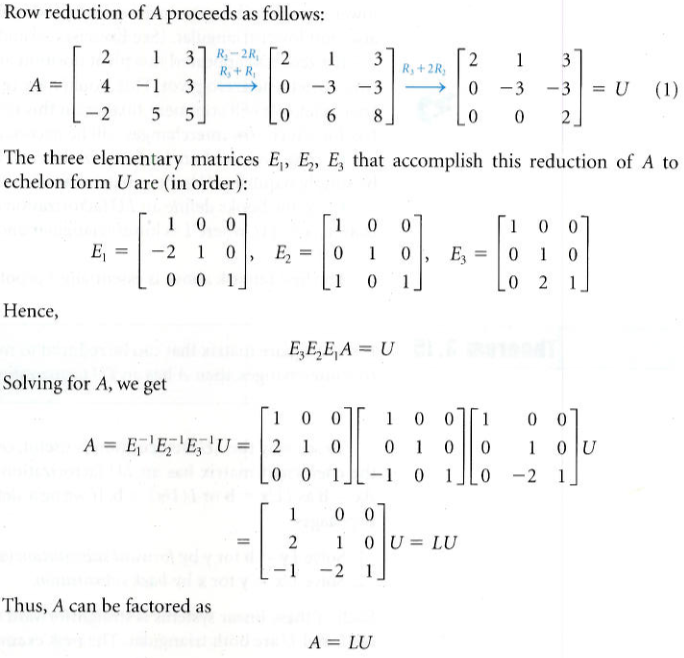
\includegraphics[scale = .5]{3}

NOTE: The row multipliers used in the preceding example are the entries of $L$ that are below its diagonal.

\subsection*{$P^TLU$ Factorization}
This method is an alternative form of the $LU$ factorization in which it handles row changes during Gaussian elimination. P is called the \textbf{permutation matrix}.\\*

Let $A$ be a square matrix. A factorization of $A$ as $A$ = $P^TLU$. This called a factorization of $A$.
\subsection*{Example}
Find a $P^TLU$ factorization of $A = \begin{bmatrix}
    0&0&6\\1&2&3\\2&1&4
\end{bmatrix}$.
\subsection*{Solution}
After reduing A to row echelon form, we get
$$\begin{bmatrix}
    1&2&3\\0&3&-2\\0&0&6
\end{bmatrix}$$

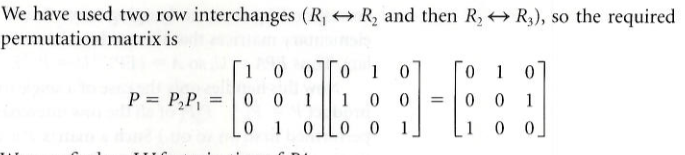
\includegraphics[scale = .5]{lu1}
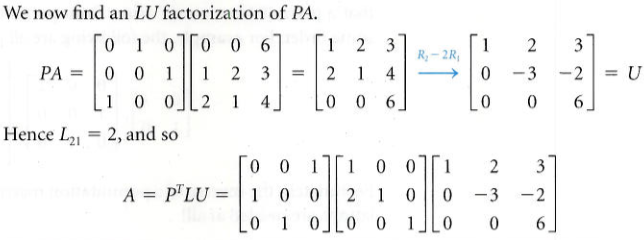
\includegraphics[scale = .5]{lu2}

\section{Subspaces, Basis, Dimension, and Rank}
\subsection*{Subspaces}
A \textbf{Subspace} of $\mathbb{R}^n$ is any collection $S$ of vectors in $\mathbb{R}^n$ such that
\begin{enumerate}
    \item The zero vector 0 in $S$.
    \item If $u$ and $v$ are in $S$, then $u+v$ is in $S$. (S is \textbf{\textit{closed under addition}}.)
    \item If $u$ is in $S$ and $c$ is a scalar, then $cu$ is in $S$. (S is \textbf{\textit{closed under scalar multiplication}}.)
\end{enumerate}
Let $v_1, v_2, \dots, v_k$ be vectors in $\mathbb{R}^n$. Then $span(v_1, v_2, \dots, v_k)$ is a subspace of $\mathbb{R}^n$.\\
Let $A$ be an $m\times n$ matrix. \begin{enumerate}
    \item The \textbf{row space} of $A$ is the subspace row(A) of $\mathbb{R}^n$ spanned by the rows of A. 
    \item The \textbf{column space} of $A$ is the subspace col(A) of $\mathbb{R}^n$ spanned by the columns of A. 
\end{enumerate}

\subsection*{Example}
Consider the matrix $A = \begin{bmatrix}
    1&-1\\0&1\\3&-3
\end{bmatrix}$. \\\begin{enumerate}[a]
    \item Determine whether $b = \begin{bmatrix}
        1\\2\\3
    \end{bmatrix}$ is the column space of $A$.
    \item Determine whether $w = \begin{bmatrix}
        4&5
    \end{bmatrix}$ is in the row space of $A$.
    \item Describe $row(A)$ and $col(A)$.
\end{enumerate}
\subsection*{Solution}
(a) We augment the matrix $[A|b]$ to determine if b is in col(A). After row reduction within the augmented matrix, 
$$\begin{bmatrix}
    1&0|&3\\0&1|&2\\0&0|0
\end{bmatrix}$$
Since the system is consistent, and has a unique solution, \textbf{b} is in $col(A)$.\\
(b) By solving the augmented matrix, $[\frac{A}{\textbf{w}}]$, and apply elementary row operations to reduce it to the form $\frac{A^\prime}{0}$, we have
$$\begin{bmatrix}
    1&0\\0&1\\0&0\\0&0
\end{bmatrix}$$ These calculations show that w is in $row(A)$.\\*
Let A be an $m\times n$ matrix. The \textbf{null space} of $A$ is the subspace of $\mathbb{R}^n$ consisting of solutions of the homogeneous linear system $Ax = 0$. It is denoted by $null(A)$.\\
\subsection*{Basis}
A \textbf{basis} for a subspace $S$ of $\mathbb{R}^n$ is a set of vectors in $S$ that \begin{enumerate}
    \item span S and 
    \item is linearly independent.
\end{enumerate}
\subsubsection*{Steps for finding the row, column, and the null spaces of a matrix A}
\begin{enumerate}
    \item Find the rref form $R$ of $A$.
    \item Use the nonzero row vectors of $R$ to form a basis for $row(A)$.
    \item Use the column vectors of $A$ that correspond to the columns of $R$ containing the leading 1s to form a basis for $col(A)$.
    \item Solve for the leading variables of $Rx = 0$ in terms of the free variables, set the free variables equal to parameters, substitute back into x, and write the result as a linear combination of \textit{f} vectors where f is the number of free variables. These f vectors form a basis for $null(A)$.
\end{enumerate}
\subsection*{Dimension and Rank}
\textbf{The Basis Theorem}\\
Let $S$ be a subspace of $\mathbb{R}^n$. Then any two bases for $S$ have the same number of vectors.\\* 

If $S$ is a subspace of $\mathbb{R}^n$, then the number of vectors in a basis for $S$ is called the \textbf{dimension} of $S$, denoted $dim S$.
Since the standard basis for $\mathbb{R}^n$ has $n$ vectors, $dim R^n = n$. 

The \textbf{rank} of a matrix $A$ is the dimension of its row and column spaces and is denoted by $rank(A)$.
The\textbf{nullity} of a matrix $A$ is the dimension of its null space and is denoted by $nullity(A)$.

\subsection*{Coordinates}
Let $S$ be a subspace of $\mathbb{R}^n$ and let $\beta = \{v_1, v_2, \dots, v_k\}$ be a basis for $S$. Let $v$ be a vector in $S$ and write $v = c_1v_1 + c_2v_2 + \dots + c_kv_k$. Then $c_1, c_2, \dots, c_k$ are called the \textbf{coordinates of v with respect to $\beta$} and the column vector
$$[v]_\beta = \begin{bmatrix}
    c_1\\c_2\\\vdots\\c_k
\end{bmatrix}$$
is called the \textbf{coordinate vector of v with respect to $\beta$}.
\subsection*{Example}
Let $\epsilon = \{e_1, e_2, e_3\}$ be the standard basis for $\mathbb{R}^3$. Find the coordinate vector of $v = \begin{bmatrix}
    2\\7\\4
\end{bmatrix}$\\ with respect to $\epsilon$.
\subsection*{Solution}
Since $v = 2e_1 + 7e_2 + 4e_3$, $$[v]_\epsilon = \begin{bmatrix}
    2\\7\\4
\end{bmatrix}$$

\section{Intro to Linear Transformations}
A \textbf{transformation} $T$ from $\mathbb{R}^n$ to $\mathbb{R}^m$ is a rule that assigns to each vector v in $\mathbb{R}^n$ a unique vector $T(v)$ in $\mathbb{R}^n$. 
\subsection*{Linear Transformations}
\begin{enumerate}
    \item $T(u+v) = T(u) + T(v)$
    \item $T(cv) = cT(v)$
\end{enumerate}
\textbf{Theorem}: Let $T: R^m\rightarrow R^n$ and $S: R^n\rightarrow R^p$ be linear transformations. Then $S\comp T: R^m\rightarrow R^p$ is a linear transformation. Moreover, their standard matricies related by\\
$[S\comp T] = [S][T]$
\textbf{Inverse Transformations}: Let $S$ and $T$ be linear transformations from $\mathbb{R}^n$ to $R_n$. Then S and T are inverse transformations if $S\comp T = I_n$ and $T\comp S = I_n$.